\section{Сэмплирование}

Зададим функцию

\begin{equation}
    f(t) = \sin(2\pi x + 1) + \sin(0.5\pi x + 4)
\end{equation}

\subsection{Сэмплирование синусов}

Построим непрерывный график: 

\begin{figure}[ht]
    \centering
    \includegraphics[width=1\textwidth]{/Users/nikolajprovorov/Yandex.Disk-368690@edu.itmo.ru.localized/Lab_5_FURRY/plots/interpolation_1/source_func.png}
    \caption{График исходной функции}
\end{figure}

\clearpage

Теперь сэмплированный вариант c шагом $\triangle t = \frac{1}{16}$

\begin{figure}[ht!]
    \centering
    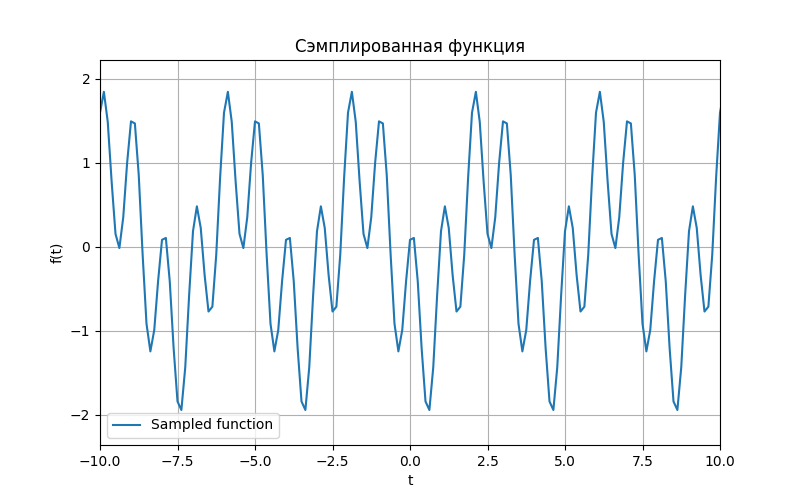
\includegraphics[width=0.8\textwidth]{/Users/nikolajprovorov/Yandex.Disk-368690@edu.itmo.ru.localized/Lab_5_FURRY/plots/interpolation_1/sampled_func.png}
    \caption{График сэмплированной функции}
\end{figure}

А вот результат их наложения:

\begin{figure}[ht!]
    \centering
    \includegraphics[width=0.8\textwidth]{/Users/nikolajprovorov/Yandex.Disk-368690@edu.itmo.ru.localized/Lab_5_FURRY/plots/interpolation_1/cmp_func.png}
    \caption{Сравнение исходной и сэмплированной функций}
\end{figure}

\clearpage

\subsubsection{Восстановление.}

Попробуем восстановить функцию после применения интерполяционной формулы. Ее вид:

\begin{equation}
    f(t) = \sum_{-\infty}^{\infty}f(t_n)sinc(2Bt-t_n)
\end{equation}

\begin{figure}[ht!]
    \centering
    \includegraphics[width=1\textwidth]{/Users/nikolajprovorov/Yandex.Disk-368690@edu.itmo.ru.localized/Lab_5_FURRY/plots/interpolation_1/cmp_func_interpolated.png}
    \caption{Сравнение исходной и восстановленной функций}
\end{figure}

Ну полулось неплохо. $B$ в данном случае был равен 8.

\clearpage

\subsubsection{Влияние шага дискретизации}

Посмотрим на влияние шага дискретизации на восстановление функции. Выберем шаг $\triangle t = \frac{1}{8}~, B = 2$

\begin{figure}[ht!]
    \centering
    \includegraphics[width=0.7\textwidth]{/Users/nikolajprovorov/Yandex.Disk-368690@edu.itmo.ru.localized/Lab_5_FURRY/plots/interpolation_2/cmp_func.png}
    \caption{Сравнение исходной и сэмплированной функций с шагом $\triangle t = \frac{1}{8}$}
\end{figure}

Восстановленная функция будет иметь вид:

\begin{figure}[ht!]
    \centering
    \includegraphics[width=0.7\textwidth]{/Users/nikolajprovorov/Yandex.Disk-368690@edu.itmo.ru.localized/Lab_5_FURRY/plots/interpolation_2/cmp_func_interpolated.png}
    \caption{Сравнение исходной и восстановленной функций с шагом $\triangle t = \frac{1}{8}$}
\end{figure}

Плоховато, давайте попробуем поменять частоту дискретизации. Пусть $\triangle t = \frac{1}{4}$

\clearpage

\begin{figure}[ht!]
    \centering
    \includegraphics[width=0.7\textwidth]{/Users/nikolajprovorov/Yandex.Disk-368690@edu.itmo.ru.localized/Lab_5_FURRY/plots/interpolation_3/cmp_func.png}
    \caption{Сравнение исходной и сэмплированной функций с шагом $\triangle t = \frac{1}{4}$}
\end{figure}

Восстановленная функция будет иметь вид:

\begin{figure}[ht!]
    \centering
    \includegraphics[width=0.7\textwidth]{/Users/nikolajprovorov/Yandex.Disk-368690@edu.itmo.ru.localized/Lab_5_FURRY/plots/interpolation_3/cmp_func_interpolated.png}
    \caption{Сравнение исходной и восстановленной функций с шагом $\triangle t = \frac{1}{4}$}
\end{figure}

Получилось отлично. Для чистоты эксперимента, попробуем выбрать $\triangle t = \frac{1}{8},~ B = 4$

\clearpage

\begin{figure}[ht!]
    \centering
    \includegraphics[width=0.8\textwidth]{/Users/nikolajprovorov/Yandex.Disk-368690@edu.itmo.ru.localized/Lab_5_FURRY/plots/interpolation_6/cmp_func.png}
    \caption{Сравнение исходной и сэмплированной функций с шагом $\triangle t = \frac{1}{8},~ B = 4$}
\end{figure}

Восстановленная функция будет иметь вид:

\begin{figure}[ht!]
    \centering
    \includegraphics[width=0.8\textwidth]{/Users/nikolajprovorov/Yandex.Disk-368690@edu.itmo.ru.localized/Lab_5_FURRY/plots/interpolation_6/cmp_func_interpolated.png}
    \caption{Сравнение исходной и восстановленной функций с шагом $\triangle t = \frac{1}{8},~ B = 4$}
\end{figure}

Снова отличный результат. Хммм, с чем же это связано? может заметить что параметр $B$ влияет на качество восстановления функции. Шаг дискретизации должен быть меньше, чем $\frac{1}{2}B$. Этот же вывод мы почерпнули из теоремы Найквиста-Шеннона-Котельникова.

\clearpage

\subsection{Сэмплирование sinus cardinalis}

Настало время синус кардиналис. Зададимся параметром $b = 5$ и функцией:

\begin{equation}
    f(t) = sinc(bt)
\end{equation}

Посмотрим на изначальный график так, как будто мы его никогда не видели:

\begin{figure}[ht!]
    \centering
    \includegraphics[width=1\textwidth]{/Users/nikolajprovorov/Yandex.Disk-368690@edu.itmo.ru.localized/Lab_5_FURRY/plots/interpolation_4/source_func.png}
    \caption{График исходной функции}
\end{figure}

\clearpage

\subsubsection{Сэмплирование синус кардиналис}

Построим сравнительный график с шагом $\triangle t = \frac{1}{8}$:

\begin{figure}[ht!]
    \centering
    \includegraphics[width=0.8\textwidth]{/Users/nikolajprovorov/Yandex.Disk-368690@edu.itmo.ru.localized/Lab_5_FURRY/plots/interpolation_4/cmp_func.png}
    \caption{Сравнение исходной и сэмплированной функций}
\end{figure}

Восстановленная функция:

\begin{figure}[ht!]
    \centering
    \includegraphics[width=0.8\textwidth]{/Users/nikolajprovorov/Yandex.Disk-368690@edu.itmo.ru.localized/Lab_5_FURRY/plots/interpolation_4/cmp_func_interpolated.png}
    \caption{Сравнение исходной и восстановленной функций}
\end{figure}

Ну, в целом, пойдет. Попробуем увеличить шаг дискретизации до $\triangle t = \frac{1}{4}$

\clearpage

Построим сравнительный график с шагом $\triangle t = \frac{1}{4}$:

\begin{figure}[ht!]
    \centering
    \includegraphics[width=0.8\textwidth]{/Users/nikolajprovorov/Yandex.Disk-368690@edu.itmo.ru.localized/Lab_5_FURRY/plots/interpolation_5/cmp_func.png}
    \caption{Сравнение исходной и сэмплированной функций}
\end{figure}

Восстановленная функция:

\begin{figure}[ht!]
    \centering
    \includegraphics[width=0.8\textwidth]{/Users/nikolajprovorov/Yandex.Disk-368690@edu.itmo.ru.localized/Lab_5_FURRY/plots/interpolation_5/cmp_func_interpolated.png}
    \caption{Сравнение исходной и восстановленной функций}
\end{figure}

Видно, что пошло хуже.

\clearpage

\subsubsection{Фурье-образ синус кардиналис и восстановленного сигнала}

Для шага дискретизации $\triangle t = \frac{1}{8}$:

\begin{figure}[ht!]
    \centering
    \includegraphics[width=0.8\textwidth]{/Users/nikolajprovorov/Yandex.Disk-368690@edu.itmo.ru.localized/Lab_5_FURRY/plots/interpolation_4/image.png}
    \caption{Фурье-образ исходного синус кардиналис}
\end{figure}

\begin{figure}[ht!]
    \centering
    \includegraphics[width=0.8\textwidth]{/Users/nikolajprovorov/Yandex.Disk-368690@edu.itmo.ru.localized/Lab_5_FURRY/plots/interpolation_4/restored_image.png}
    \caption{Фурье-образ восстановленного синус кардиналис}
\end{figure}

\clearpage

Для шага дискретизации $\triangle t = \frac{1}{4}$:

\begin{figure}[ht!]
    \centering
    \includegraphics[width=0.8\textwidth]{/Users/nikolajprovorov/Yandex.Disk-368690@edu.itmo.ru.localized/Lab_5_FURRY/plots/interpolation_5/image.png}
    \caption{Фурье-образ исходного синус кардиналис}
\end{figure}

\begin{figure}[ht!]
    \centering
    \includegraphics[width=0.8\textwidth]{/Users/nikolajprovorov/Yandex.Disk-368690@edu.itmo.ru.localized/Lab_5_FURRY/plots/interpolation_5/restored_image.png}
    \caption{Фурье-образ восстановленного синус кардиналис}
\end{figure}

\clearpage

\subsubsection{Выводы}

Лучше всего функция восстанавливается когда шаг дискретизации меньше, чем $\frac{1}{2}B$. С образом тоже все нормально. Мы знаем, что образ синус кардиналиса - прямоугольная волна. Она и получилась. Правда из сэмплированной образ получается периодическим, тк функция дискретная. Но в целом, все нормально.